

% Methodology Chapter: Expanded and Enhanced
\subsection*{1. Introduction to Threat Modeling Methodology}
Threat modeling is most effective when approached as a systematic, repeatable process that integrates technical rigor with business context\cite{shostack2014,uceda2015,owasp}. This chapter provides a detailed methodology, technical definitions, and practical tools for organizations seeking to build resilient systems and manage risk proactively.

\subsection*{2. Step-by-Step Threat Modeling Process}
	extbf{Step 1: Identify Assets}
The first step in threat modeling is to identify all assets that require protection. Assets include data, systems, credentials, intellectual property, and any other resources of value to the organization\cite{nist800154}. A comprehensive asset inventory is created using interviews, documentation reviews, and architecture diagrams. This inventory forms the foundation for subsequent analysis, ensuring that all critical resources are considered in the threat model.

	extbf{Step 2: System Decomposition}
System decomposition involves breaking down the application into its constituent components, data flows, and trust boundaries\cite{shostack2014}. Data Flow Diagrams (DFDs) are used to visualize how information moves within the system and where controls are applied. This step helps teams understand the architecture, identify potential entry points for attackers, and pinpoint areas that require additional scrutiny.

	extbf{Step 3: Identify Threats}
Threats are potential events or actions that could cause harm to assets\cite{owasp}. Security teams apply frameworks such as STRIDE or PASTA to each component and data flow, using checklists and attack trees to ensure comprehensive coverage. This analysis enables organizations to anticipate how adversaries might target the system and what tactics they might employ.

	extbf{Step 4: Identify Vulnerabilities}
Vulnerabilities are weaknesses that can be exploited by threats\cite{nist800154}. Teams use vulnerability databases (e.g., CVE, NVD), automated scanners, and code reviews to identify and document vulnerabilities. This step is critical for prioritizing remediation efforts and ensuring that the most significant risks are addressed first.

	extbf{Step 5: Assess Risks}
Risk assessment combines the likelihood and impact of a threat exploiting a vulnerability\cite{uceda2015}. Organizations use risk matrices and scoring systems (such as DREAD and CVSS) to evaluate and prioritize risks. This structured approach supports informed decision-making and resource allocation.

	extbf{Step 6: Define and Prioritize Mitigations}
Mitigations are security controls designed to reduce risk\cite{owasp}. Teams develop and prioritize controls based on business impact, cost, and feasibility. This step ensures that security investments are aligned with organizational goals and that resources are used effectively.

	extbf{Step 7: Document and Communicate}
Documentation is essential for making the threat model accessible, actionable, and up-to-date\cite{shostack2014}. Teams create detailed reports with diagrams, tables, and recommendations, sharing them with stakeholders and updating them as the system evolves. Effective communication ensures that everyone understands the risks and the steps being taken to mitigate them.

\subsection*{3. Templates, Tools, and Best Practices}
To support the threat modeling process, organizations use a variety of templates and tools, including asset inventory templates, DFD and architecture diagram examples, threat checklists (such as STRIDE and OWASP Top 10), risk matrix templates, and mitigation tracking spreadsheets. These resources help standardize the process and ensure consistency across projects. Modern tools such as the Microsoft Threat Modeling Tool, OWASP Threat Dragon, and custom spreadsheets are widely used in industry.

\subsection*{4. Workflow Diagram}
The following diagram illustrates the threat modeling workflow, from asset identification to mitigation:
\begin{figure}[H]
	\centering
	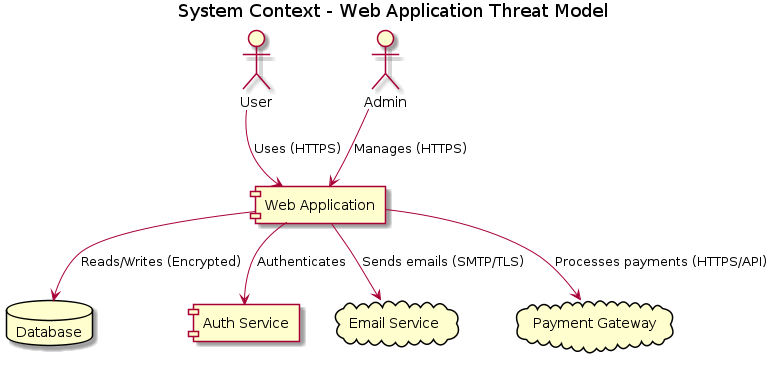
\includegraphics[width=0.7\textwidth]{images/system-context}
	\caption{Threat Modeling Workflow: From Asset Identification to Mitigation\cite{shostack2014}}
\end{figure}

\subsection*{5. Academic Perspective and Further Reading}
For deeper understanding, refer to:
\begin{itemize}
	\item Adam Shostack, "Threat Modeling: Designing for Security" (Wiley, 2014)
	\item Tony UcedaVélez and Marco M. Morana, "Risk Centric Threat Modeling" (Wiley, 2015)
	\item NIST SP 800-154: Guide to Data-Centric System Threat Modeling
	\item OWASP Threat Modeling Cheat Sheet
\end{itemize}
